\documentclass{standalone}

\usepackage{pgfplots}
\usetikzlibrary{intersections}

\begin{document}

\newcommand*{\ShowIntersectionWithSinAbs}{
\fill 
    [name intersections={of=DroiteK and SinAbs, name=i, total=\t}] 
    [red, opacity=1, every node/.style={above left, black, opacity=1}] 
    \foreach \s in {1,...,\t}{
        \ifodd \s 
        {}
        \else
        (i-\s) circle (2pt) node [above] {\s} 
        \fi 
        };
}
\newcommand*{\ShowIntersectionWithCosAbs}{
\fill 
    [name intersections={of=DroiteK and CosAbs, name=i, total=\t}] 
    [blue, opacity=1, every node/.style={above left, black, opacity=1}] 
    \foreach \s in {1,...,\t}{
        \ifodd \s 
        (i-\s) circle (2pt) node [above] {\s} 
        \fi 
        };
}


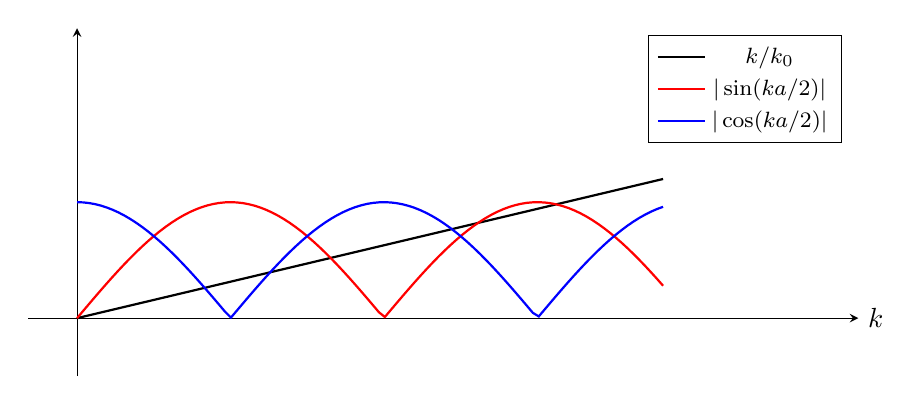
\begin{tikzpicture}
    \begin{axis}[
        xmax = 8,
        xmin = -0.5,
        ymin = -0.5,
        ymax = 2.5,
        axis lines = middle,
        xlabel style = {right},
        ylabel style = {above},
        xlabel = {$k$},
        width=\linewidth,
        height = 6cm,
        ticks = none,
        ]
    
\addplot[name path global=DroiteK, mark=none, domain=0:6, thick]%
{x/5};%

\addplot [red, thick, name path global=SinAbs, domain = 0:6, samples = 100]  {abs(sin(deg(x)))} ;%

\addplot [blue, thick, name path global=CosAbs, domain = 0:6, samples = 100]  {abs(cos(deg(x)))};%
\ShowIntersectionWithSinAbs% Works
\ShowIntersectionWithCosAbs% Works
\legend{\footnotesize $k/k_0$, \footnotesize $|\sin(ka/2)|$, \footnotesize $|\cos(ka/2)|$}
\end{axis} 
\end{tikzpicture}
\end{document}